\section{Задание 3}

Ввести длину и ширину в поля формы и определить площадь этого прямоугольника. Площадь должна вычисляться по нажатию кнопки.

\begin{center}
  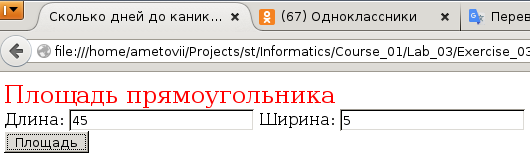
\includegraphics{img/Exercise_03/01.png}
  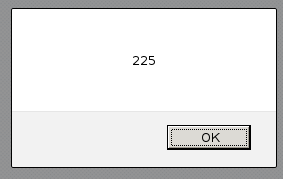
\includegraphics{img/Exercise_03/02.png}
\end{center}

Исходный код \verb|exercise_03.html|:

\begin{verbatim}
<!doctype html>
<html>
  <head>
    <title>Сколько дней до каникул?</title>
    <meta charset='utf-8' />
  </head>
  <body>
    <font color="red" size="5">Площадь прямоугольника</font><br>
    Длина: <input id="inputLength"></input>
    Ширина: <input id="inputWidth"></input> <br>
    <button onclick="calculateYardage()">Площадь</button>
    <script>
      function calculateYardage(){
	  var length=document.getElementById("inputLength");
	  var width=document.getElementById("inputWidth");
	  alert(length.value*width.value);
      }
    </script>
  </body>
</html>
\end{verbatim}
